\section{Control}
In the previous section, mathematical modeling of the \scps was discussed. Their control strategies and results are shown in this section. Based on the models in section \ref{section_modeling}, the \anta was controlled to follow the desired position, which is a function of time. We will now call this \apcnospace.

\subsection{Basic Strategy for the \APC}
By assuming that $\ddot{\theta}$ and $\dot{\theta}$ are small enough, we could observe correlation between $\theta$ and $T_{1}$, $T_{2}$ from \eqref{EqAnta} as \eqref{simple_assume}.
\begin{equation} \label{simple_assume}
\theta = \frac{c}{2kr}(T_{1}-T_{2}).
\end{equation}
By multiplying Laplace transformed equations of \eqref{thermo-electrical_model} and \eqref{simple_assume}, we could discover transfer function of $P$ and $\theta$ as \eqref{apc_transfer}.

\begin{equation} \label{apc_transfer}
\frac{\theta(s)}{P(s)} = \frac{c/2kr}{C_{th}s+\lambda}.
\end{equation}
Therefore, the process of controlling $\theta$ into $\theta_{ref}$ by applying constant power can be shown as block diagram in Fig.\ref{AntaControl_constant}. 

In this situation, $K_{\theta,P}$ is constant. By applying constant power to only one of the muscles, $\theta$ at steady state was measured. Linear fitting of Fig.\ref{KthetaP} gave us the following constant.

\begin{equation}
K_{\theta,P} = \SI{0.185}{\watt\per\degree}. \notag
\end{equation}
For the fast and precise control, a lead compensator was added and subsequently, feedback, and feedforward control were applied, as can be seen in Fig.\ref{position_open_loop}, \ref{position_closed_loop}.

\begin{figure}[t]
	\centering
	\begin{minipage}{0.30\textwidth}
		\begin{subfigure}{\linewidth}
			\centering
			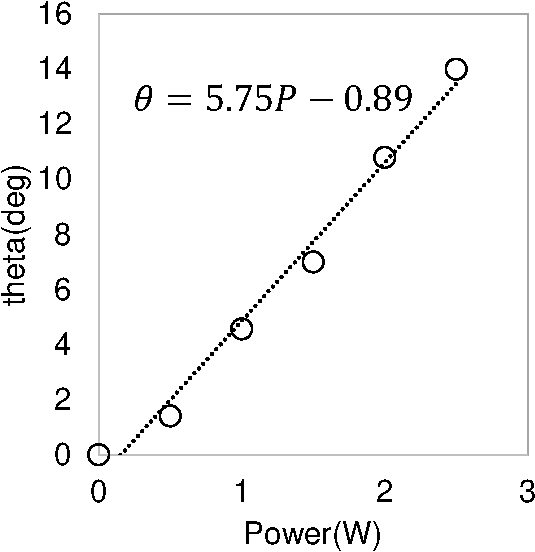
\includegraphics[width=\linewidth]{K_theta_P_v4-cropped.pdf}
			\caption{\label{KthetaP}}
		\end{subfigure}
	\end{minipage}%
	\begin{minipage}{0.6\textwidth}
		\centering
		\begin{subfigure}{0.55\linewidth}
			\centering
			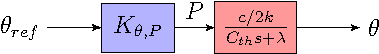
\includegraphics[width=\linewidth]{Diagram(v4)_position_constant.pdf}
			\caption{\label{AntaControl_constant}}
		\end{subfigure}
		
		\begin{subfigure}{0.73\linewidth}
			\centering
			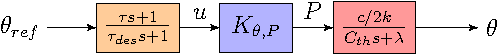
\includegraphics[width=\linewidth]{Diagram(v4)_position_openloop.pdf}
			\caption{\label{position_open_loop}}
		\end{subfigure}
		
		\begin{subfigure}{\linewidth}
			\centering
			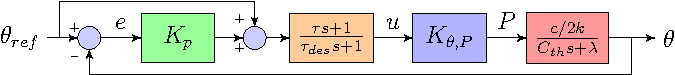
\includegraphics[width=\linewidth]{Diagram(v4)_position_feedback.pdf}
			\caption{\label{position_closed_loop}}
		\end{subfigure}
	\end{minipage}
	\caption[Block diagrams for the \apc]{\subref{KthetaP} There's a linear relationship between applied power and $\theta$ at steady state. \subref{AntaControl_constant} Process of obtaining desired angle with constant power. \subref{position_open_loop} Process of the \apc including a lead compensator. \subref{position_closed_loop} Process of the \apc including feedback and feedforward.}
	\label{anta_position_diagrams}
\end{figure}


\subsection{Antagonistic Position Control Strategy}
In this section, we aim to make a simple sin wave motion of the \anta as \eqref{theta_ref}. By doing this, we could check the possibility of the \apc for any complicated motion. Basically, according to the equation \eqref{simple_assume}, we could increase $\theta$ by heating muscle 1 and decrease $\theta$ by heating muscle 2. Therefore, we used a strategy shown in Table.\ref{table_apc_basic}
%By assuming that $\ddot{\theta}$ and $\dot{\theta}$ is small enough, \eqref{EqAnta} can be approximated into \eqref{EqAngleTempDiff}.

%\begin{equation}\label{EqAngleTempDiff}
%\theta=\frac{c}{2kr}(T_1-T_2)
%\end{equation}



\begin{equation}\label{theta_ref}
\theta_{ref}(t)=(\SI{9}{\degree})\sin(2\pi 0.025t)
\end{equation}

\begin{table}[b]
	\caption{Basic strategy for the \apc.}
	\label{table_apc_basic}
	\begin{center}
		\begin{tabular}{c||c|c|c|c}
			\hline
			Time(s) & 0-10 & 10-20 & 20-30 & 30-40 \\
			\hline
			Muscle 1 & Heat & Keep & Keep & Heat \\
			Muscle 2 & Keep & Heat & Heat & Keep \\
			\hline
			$\theta$ & increase & decrease & decrease & increase \\
			\hline
		\end{tabular}
	\end{center}
\end{table}

Since the Laplace transformation of \eqref{theta_ref} is too complicated, we used an approximation shown in \eqref{theta_ref_approx} by dividing \eqref{theta_ref} into 12 steps. In this case, demanded power can be calculated as \eqref{power_derived} since $n=12$.
\footnote{In equation \eqref{power_derived}, $\theta_{ref,pre}$ is a value of $\theta_{ref}$ in the previous step. Also, $t$ is elapsed time after starting a new step.}
\footnote{$U(t)$ is unitary step function.}
\begin{equation} \label{theta_ref_approx}
\begin{aligned} 
%\theta_{ref}(t) = \sum_{i=0}^{n-1}{(\theta_{ref,i+1}-\theta_{ref,i})U(t-i\Delta T)} 
\theta_{ref}(t) & = \sum_{i=0}^{n-1}{(\theta_{ref,i+1}-\theta_{ref,i})U(t-i\Delta T)} \\
& = \sum_{i=0}^{n-1}{\left(\sin{\frac{2(i+1)\pi}{n}}-\sin{\frac{2i\pi}{n}}\right)U\left(t-40\frac{i}{n}\right)}. \\
\end{aligned}
\end{equation}

\begin{equation} \label{power_derived}
P(t)=\theta_{ref}K_{\theta,P}\left(1+\left(\frac{\theta_{ref}-\theta_{ref,pre}}{\theta_{ref}}\right)\left(\frac{\tau}{\tau_{des}}-1\right)e^{-\frac{t}{\tau_{des}}}\right).
\end{equation}

 %Through these steps, we can do \apc as a sin wave form.

%\begin{figure}[t]
%	\centering
%	\begin{subfigure}[t]{0.44\textwidth}
%		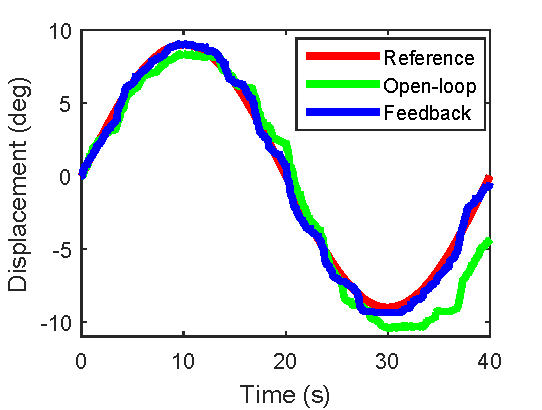
\includegraphics[width=\textwidth]{SinWave.pdf}
%		\caption{\label{positionControl_sin}}
%	\end{subfigure}%
%	\begin{subfigure}[t]{0.50\textwidth}
%		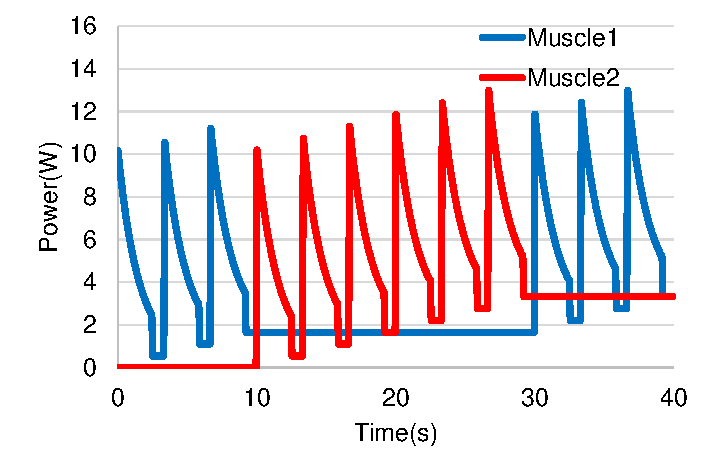
\includegraphics[width=\textwidth]{Openloop_power_graph_v2.pdf}
%		\caption{\label{positionControl_sin_power}}
%	\end{subfigure}
%	\caption[\Apc by only heating]{\subref{positionControl_sin} Measured arm's angular position in function of time. Feedback control had smaller error than open-loop control. \subref{positionControl_sin_power} Used power of each \scpnospace s(Open loop)}
%	\label{positionControl}
%\end{figure}

%\clearpage

\subsection{Sustainable Antagonistic Position Control Strategy}\label{section_simulation}
In the previous section, the method for making sin wave motion was discussed. However, since the temperature of the muscles in the initial state and final state is significantly different, it won't be sustainable because the temperature will keep going up. Therefore, we needed to make the temperature of the initial state and final state the same. This could be done by cooling the muscle during the last 1/4 period of sin wave, as shown in Table \ref{table_apc_sustain}.

\begin{table}[b]
	\caption{Sustainable \apc strategy.}
	\label{table_apc_sustain}
	\begin{center}
		\begin{tabular}{c||c|c|c|c|c|c|c}
			\hline
			Time(s) & 0 & 0-10 & 10-20 & 20-30 & \multicolumn{2}{|c|}{30-40} & 40 \\
			\hline
			Muscle 1 & $T_0$ & Heat & Keep & Keep & Weakly Cool & Heat & $T_0$ \\
			Muscle 2 & $T_0$ & Keep & Heat & Heat & Strongly Cool & Keep & $T_0$ \\
			\hline
			$\theta$ & $0^{\circ}$ & increase & decrease & decrease & \multicolumn{2}{|c|}{increase} & $0^{\circ}$ \\
			\hline
		\end{tabular}
	\end{center}
\end{table}

\tocless \subsubsection{Demonstration - Two Period Sin Wave}
First, we demonstrated open-loop control of cooling speed. Two-period sin wave control was done, and cooling was done during $t=$\SI{40}{\second} - \SI{50}{\second}.\footnote{This slightly differs from the Table \ref{table_apc_sustain}.} In order to cool as much as possible, muscle 2 was cooled for all the time, and muscle 1 was `weakly' cooled by repeatedly opening and closing the solenoid valve. As a result, we got an rms error 26.6\% for the open-loop control, and 6.7\% for the closed-loop control.(Fig.\ref{sustain_demo})

%After the demonstration, we concluded that an appropriate time for cooling will be \SI{30}{\second}-\SI{40}{\second}, not \SI{40}{\second} - \SI{50}{\second}. It is because 
\begin{figure}[t]
	\centering
	\begin{subfigure}[t]{0.45\textwidth}
		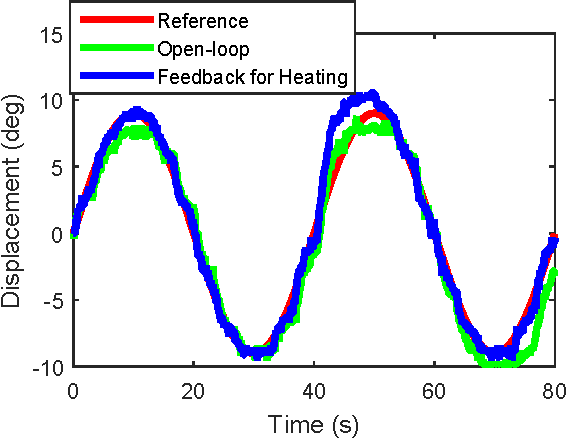
\includegraphics[width=\textwidth]{SinWave_cooling-cropped.pdf}
		\caption{\label{SinWave_cooling}}
	\end{subfigure}
	~
	\begin{subfigure}[t]{0.44\textwidth}
		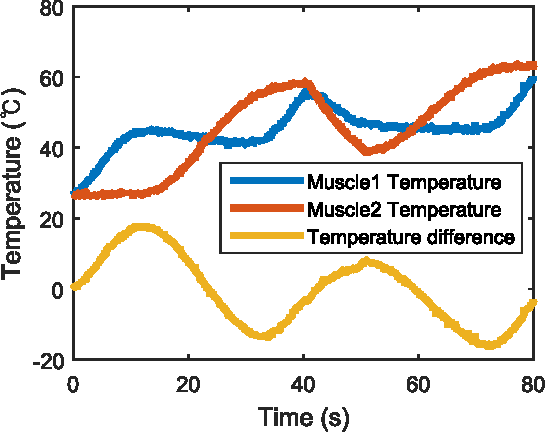
\includegraphics[width=\textwidth]{SinWaveC_T-cropped.pdf}
		\caption{\label{Sinwave_C_T}}
	\end{subfigure}
	\caption[Sustainable open-loop \apc demonstration]{\subref{SinWave_cooling} Arm's angle in function of time. \subref{Sinwave_C_T} Temperature of two muscles in function of time. We checked that sustainable \apc is possible by cooling for some time.}
	\label{sustain_demo}
\end{figure}

\tocless \subsubsection{Simulation - Feedback Control of Thermal Conductivity}


Integrating \eqref{dynamic_calculation_tau} and \eqref{lambda_control}, we could gain \eqref{tau_modification}.
\begin{equation} \label{tau_modification} 
\begin{aligned} 
\tau & = \frac{C_{th}}{\lambda} \\
& = \frac{1.81}{0.77\cdot r + 0.10}. \\ 
\end{aligned}
\end{equation}
Also, by differentiating \eqref{simple_assume} and \eqref{theta_ref} with respect to time, we could draw \eqref{theta_diff} where $t$ refers to time elapsed since $t=\SI{30}{\second}$.

\begin{equation} \label{theta_diff}
\begin{aligned} 
\frac{d\theta}{dt} & = \frac{c}{2kr}\cdot\frac{d}{dt}(T_{1}-T_{2}) \\
& = 9^{\circ}(2\pi\cdot 0.025)\sin{2\pi\cdot 0.025t}.
\end{aligned}
\end{equation}
What we had to do was to decrease $(T_{1}+T_{2})/2$, so we will use equation \eqref{diff_t1+t2}. Constant $\alpha$ was carefully determined by several simulations.
\begin{equation} \label{diff_t1+t2}
\frac{d}{dt}(T_{1}+T_{2}) = -\alpha(T_{1}+T_{2}-2T_{ambient})
\end{equation}
Therefore, by using \eqref{thermo-electrical_model} for the each muscles, we could calculate needed $\lambda_{1}$, $\lambda_{2}$. The block diagram which represents feedback control of thermal conductivities is shown in Fig.\ref{diagram_sustainable}.

\begin{figure}[t]
	\centering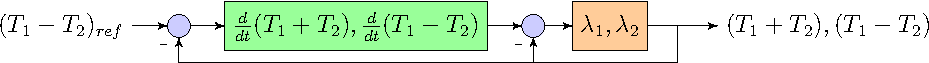
\includegraphics[width=\textwidth]{Diagram(v4)_sustainable.pdf}
	\caption{Block diagram for the sustainable \apcnospace.}
	\label{diagram_sustainable}
\end{figure}

To make sustainable \apc possible, $\lambda$ must be between $\SI{0.25}{\watt\per\degreeCelsius}$ and $\SI{0.60}{\watt\per\degreeCelsius}$  all the time, according to \eqref{lambda_control}. Therefore, possibility of this control strategy was verified by thermal simulation.
%We can guess that $\lambda_{1}$ have to decrease and $\lambda_{2}$ have to increase. 

We needed to make $\lambda_{1}$ and $\lambda_{2}$ to reach its limit as late as possible. This was determined by constant $\alpha$. 
In Fig.\ref{Sinwave_C_T}, we could observe that two of the muscles' average temperatures had increased approximately \SI{30}{\degreeCelsius}. This means that we had to cool down the average temperature at least \SI{30}{\degreeCelsius}. 

Simulation was carefully done by applying \eqref{thermo-electrical_model} and \eqref{EqAnta}, using the constants we got in section \ref{section_modeling}. The differential equation was numerically solved with 4th order Runge-Kutta method. 

Through several simulations, we have concluded that $\alpha = 0.25$ is the best. The result of simulation with this value is shown in Fig.\ref{cool_simulation}. With initial temperature from Fig.\ref{Sinwave_C_T}, {\it i.e.} $T_{1}=\SI{40}{\degreeCelsius}$ and $T_{2}=\SI{55}{\degreeCelsius}$ at $t=\SI{30}{\second}$, the required thermal conductivity slightly hit the maximum limit. Also, the average temperature didn't decrease over \SI{30}{\degreeCelsius}. Therefore, the temperature will increase in this state.

Once average temperature increases, it will be easier to cool the muscles because $dT/dt \propto (T-T_{amb})$. Simulation was done again with initial temperature $T_{1}=\SI{85}{\degreeCelsius}$ and $T_{2}=\SI{100}{\degreeCelsius}$ at $t=\SI{30}{\second}$. In this time, there was a dramatic decrease of average temperature. (Fig.\ref{cool_control_100}) Also, required thermal conductivity hit the limit after cooling two of the muscles in full degree. After reaching the desired amount of cooling, we could maintain $\theta_{ref}$ by switching cooling to heating. Finally, we could conclude that feedback cooling control is possible, so that we were able to make \apc highly sustainable.

\begin{figure}[t]
	\centering
	\begin{subfigure}[t]{0.45\textwidth}
		\centering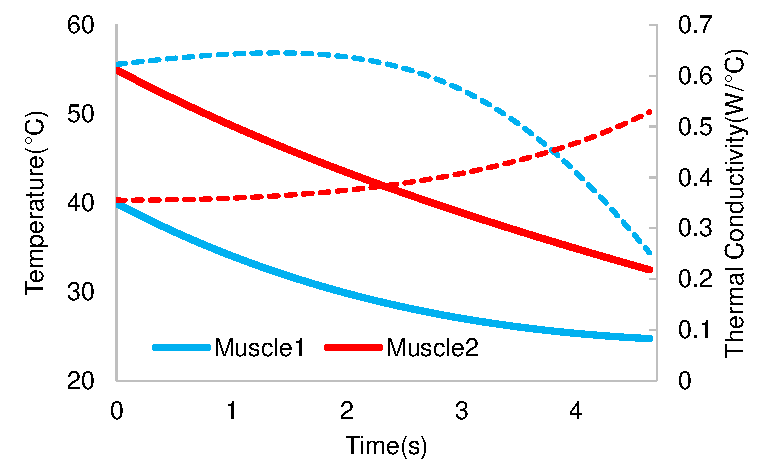
\includegraphics[width=\textwidth]{cool_control_T+lambda_v2.pdf}
		\caption{\label{cool_control}}
	\end{subfigure}%
	\begin{subfigure}[t]{0.45\textwidth}
		\centering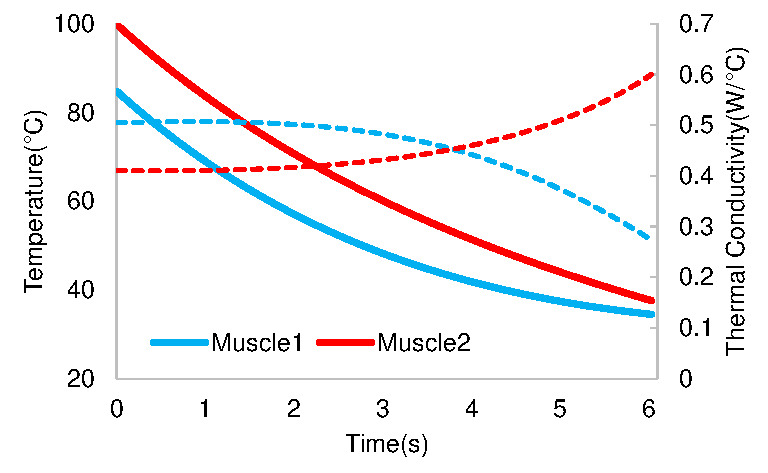
\includegraphics[width=\textwidth]{cool_control_T+lambda_100_85_v2.pdf}
		\caption{\label{cool_control_100}}
	\end{subfigure}
	\caption[Sustainable closed-loop \apc simulation]{\subref{cool_control} Temperature and thermal conductivity of two muscles in function of time after $t=\SI{30}{\second}$. Temperature is in full lines, and thermal conductivity is in broken lines. \subref{cool_control_100} Thermal conductivity of two muscles in function of time. }
	\label{cool_simulation}
\end{figure}




